\documentclass[11pt,a4paper]{article}

% ---------------------------------------------------------------------------
\usepackage[utf8]{inputenc}
\usepackage[margin=2.5cm]{geometry}
\usepackage{amsmath,amssymb,amsthm}
\usepackage{enumitem}
\usepackage{booktabs}
\usepackage{xcolor}
\usepackage{tikz}
\usepackage{listings}
\usepackage{fancyhdr}
\usepackage[hidelinks]{hyperref}

\definecolor{accent}{HTML}{E4572E}
\definecolor{edgegray}{HTML}{9AA1AE}
\definecolor{codebg}{HTML}{F6F8FA}
\definecolor{codekw}{HTML}{8250DF}
\definecolor{codecm}{HTML}{6E7781}
\definecolor{codestr}{HTML}{0A3069}

\lstset{
  language=Python,
  basicstyle=\ttfamily\footnotesize,
  keywordstyle=\color{codekw}\bfseries,
  commentstyle=\color{codecm}\itshape,
  stringstyle=\color{codestr},
  backgroundcolor=\color{codebg},
  numbers=left, numberstyle=\tiny\color{codecm}, numbersep=8pt,
  frame=single, rulecolor=\color{codebg},
  showstringspaces=false, breaklines=true, columns=fullflexible,
  xleftmargin=1.5em, framexleftmargin=1.5em,
}

\newtheorem{theorem}{Theorem}[section]
\newtheorem{proposition}[theorem]{Proposition}
\newtheorem{lemma}[theorem]{Lemma}
\newtheorem{conjecture}[theorem]{Conjecture}
\theoremstyle{definition}
\newtheorem{definition}[theorem]{Definition}
\newtheorem{example}[theorem]{Example}
\newtheorem{remark}[theorem]{Remark}

\pagestyle{fancy}
\fancyhf{}
\fancyhead[L]{\small Erd\H{o}s--Gy\'arf\'as Conjecture}
\fancyhead[R]{\small University of Bucharest}
\fancyfoot[C]{\thepage}

\newcommand{\C}[1]{C_{#1}}
\newcommand{\doi}[1]{\href{https://doi.org/#1}{doi:#1}}

% ---------------------------------------------------------------------------
\begin{document}

\begin{titlepage}
  \centering
  \vspace*{3cm}
  {\Huge\bfseries The Erd\H{o}s--Gy\'arf\'as Conjecture\par}
  \vspace{0.8cm}
  {\Large Cycles of Power-of-Two Length, the Markstr\"om Graph,\\
   and Computational Approaches\par}
  \vspace{2.5cm}
  \begin{tabular}{rl}
    \textbf{Course:}     & Formal Languages and Automata (LFA) \\
    \textbf{Faculty:}    & Faculty of Mathematics and Computer Science \\
    \textbf{University:} & University of Bucharest \\[0.6em]
    \textbf{Author:}     & Ionescu-Telibasa Denis-Alexandru \\
    \textbf{Group:}      & 143 \\
    \textbf{Year:}       & First Year, Computer Science \\[0.6em]
    \textbf{Date:}       & June 3, 2026 \\
    \textbf{Revised:}    & October 2026
  \end{tabular}
  \vfill
  {\small Code and figures: \url{https://github.com/DenWick/erdos-gyarfas}\par}
\end{titlepage}

\tableofcontents
\newpage

% ===========================================================================
\section*{Abstract}
\addcontentsline{toc}{section}{Abstract}

The Erd\H{o}s--Gy\'arf\'as Conjecture (1995) asserts that every graph with
minimum degree at least $3$ contains a cycle whose length is a power of $2$.
Despite its elementary statement, the conjecture remains open. This paper
surveys its origin, develops the necessary graph-theoretic background, and
summarises what is currently known. We give a full description of the
Markstr\"om graph, the smallest planar cubic graph with no cycle of length $4$
or $8$, and verify its properties with an exact cycle-search program, whose
implementation and correctness tests we present. We close with a discussion of
why the conjecture is interesting from the point of view of formal language
theory.

\paragraph{Note on this revision.}
This version corrects the June 2026 submission. The construction of the
Markstr\"om graph, the cycle-search algorithm, and several stated results were
wrong in the original and have been replaced by statements that are either
proved here, verified by the accompanying program, or taken directly from the
cited literature.

% ===========================================================================
\section{Historical Background and Motivation}

\subsection{Paul Erd\H{o}s and the Art of Conjecture}

Paul Erd\H{o}s (1913--1996) was one of the most prolific mathematicians of the
twentieth century, with around 1{,}500 papers across combinatorics, number
theory, graph theory and probability. He worked collaboratively, travelled
constantly, and often attached small monetary prizes to problems he found
important. The \emph{Erd\H{o}s number}, the collaborative distance from him,
has become part of mathematical culture.

\subsection{Andr\'as Gy\'arf\'as}

Andr\'as Gy\'arf\'as is a Hungarian combinatorialist known for his work in
Ramsey theory, graph colouring and the structure of cycles in graphs. He and
Erd\H{o}s formulated the conjecture discussed here in 1995; it appeared in
print in Erd\H{o}s' 1997 problem paper~\cite{erdos1997}, and is listed today as
Problem~\#64 in the Erd\H{o}s problems database~\cite{erdosproblems}.

\subsection{Why Powers of Two?}

Minimum degree $3$ is a weak condition, but it already forces rich cycle
structure. It forces cycles, and in fact even cycles (Proposition~\ref{prop:even}).
It does not force any \emph{particular} even length: there are cubic graphs
with no $\C4$ (for example the Petersen graph), and with neither $\C4$ nor
$\C8$ (the Markstr\"om graph of Section~\ref{sec:markstrom}). The powers of
two form a sparse, infinite set of lengths, and the conjecture asks whether
minimum degree $3$ is already enough to hit it.

% ===========================================================================
\section{Graph-Theoretic Preliminaries}

\subsection{Basic Definitions}

\begin{definition}[Graph]
A \emph{simple graph} is a pair $G=(V,E)$ where $V$ is a finite set of
vertices and $E\subseteq\binom{V}{2}$ is a set of edges. We write $n=|V|$
and $m=|E|$.
\end{definition}

\begin{definition}[Degree]
The \emph{degree} $\deg(v)$ of $v\in V$ is the number of edges incident to
$v$. The \emph{minimum degree} of $G$ is $\delta(G)=\min_{v\in V}\deg(v)$.
\end{definition}

\begin{definition}[Cycle]
A \emph{cycle} of length $k\ge3$, written $\C k$, is a sequence of $k$
\emph{distinct} vertices $v_1,\dots,v_k$ such that $v_iv_{i+1}\in E$ for all
$i$, indices taken modulo $k$.
\end{definition}

\begin{definition}[Power-of-two cycle]
A cycle is a \emph{power-of-two cycle} if its length lies in
$\{4,8,16,32,\dots\}=\{2^k : k\ge2\}$.
\end{definition}

\begin{definition}[Regular graph]
$G$ is \emph{$k$-regular} if $\deg(v)=k$ for every $v$; $3$-regular graphs
are called \emph{cubic}.
\end{definition}

\subsection{Classical Results on Cycle Lengths}

\begin{theorem}[Dirac, 1952~\cite{dirac}]
If $n\ge3$ and $\delta(G)\ge n/2$, then $G$ contains a Hamiltonian cycle.
\end{theorem}

\begin{theorem}[Bondy--Simonovits, 1974~\cite{bondy-simonovits}]
For every $k\ge2$ there is a constant $c_k$ such that every graph on $n$
vertices with more than $c_k\,n^{1+1/k}$ edges contains a cycle of length
exactly $2k$.
\end{theorem}

These illustrate two paradigms: large minimum degree forcing long cycles, and
edge density forcing a prescribed even length. The Erd\H{o}s--Gy\'arf\'as
Conjecture belongs to a third: a \emph{small, constant} minimum degree forcing
some length from an infinite, sparse family.

% ===========================================================================
\section{The Erd\H{o}s--Gy\'arf\'as Conjecture}

\subsection{Statement}

\begin{conjecture}[Erd\H{o}s--Gy\'arf\'as, 1995]\label{conj:eg}
Every graph $G$ with $\delta(G)\ge3$ contains a cycle whose length is a power
of $2$.
\end{conjecture}

\begin{example}[The degree bound is tight]
The odd cycle $\C{2k+1}$ has $\delta=2$ and its only cycle has odd length, so
it contains no power-of-two cycle. Hence $\delta\ge3$ cannot be weakened to
$\delta\ge2$.
\end{example}

\begin{remark}
Finiteness matters: an infinite tree in which every vertex has degree $3$ has
no cycles at all~\cite{erdosproblems}.
\end{remark}

\subsection{A Warm-Up: Minimum Degree 3 Forces an Even Cycle}

The following classical argument shows that $\delta\ge3$ does force
\emph{some} even cycle. It is instructive to see exactly where it stops short
of a power of two.

\begin{proposition}\label{prop:even}
Every graph with $\delta(G)\ge3$ contains a cycle of even length.
\end{proposition}

\begin{proof}
Let $P=x_0x_1\cdots x_\ell$ be a longest path in $G$. Every neighbour of
$x_0$ lies on $P$, since otherwise $P$ could be extended. As
$\deg(x_0)\ge3$, the vertex $x_0$ has neighbours $x_1$, $x_i$ and $x_j$ with
$1<i<j$. These give three cycles:
\[
  x_0x_1\cdots x_ix_0 \;(\text{length } i+1),\qquad
  x_0x_1\cdots x_jx_0 \;(\text{length } j+1),\qquad
  x_0x_i\cdots x_jx_0 \;(\text{length } j-i+2).
\]
If the first two both have odd length, then $i$ and $j$ are both even, so
$j-i+2$ is even. In every case one of the three cycles is even.
\end{proof}

The proof controls the \emph{parity} of a cycle but says nothing about its
exact length, which is precisely what the conjecture needs.

\subsection{Current Status}

The conjecture is open. The following partial results are known (see
\cite{erdosproblems} for a maintained list).

\begin{itemize}[leftmargin=*]
  \item \textbf{3-connected cubic planar graphs.} Heckman and
        Krakovski~\cite{heckman-krakovski} proved the conjecture for this
        class. The proof is long and partly computer-assisted, using the
        discharging method.
  \item \textbf{Planar claw-free graphs:} proved by Daniel and Shauger (2001)~\cite{erdosproblems}.
  \item \textbf{Large minimum degree.} Liu and Montgomery~\cite{liu-montgomery}
        proved that the conclusion holds whenever the minimum degree is at
        least some (very large) absolute constant. Erd\H{o}s and Gy\'arf\'as had
        in fact suspected the opposite: that for every $r$ there is a graph
        with $\delta\ge r$ and no power-of-two cycle. Liu and Montgomery
        disproved that stronger suspicion. The gap between their constant and
        $3$ is what remains open.
  \item \textbf{Restricted classes:} the conjecture is known for several
        families of Cayley graphs, for $P_8$-free and $P_{10}$-free graphs,
        and for graphs of diameter~$2$~\cite{erdosproblems}.
\end{itemize}

\paragraph{Size of a counterexample.}
Exhaustive computer searches by Royle and Markstr\"om show that a
counterexample must have at least $17$ vertices, and a \emph{cubic}
counterexample at least $30$ vertices~\cite{markstrom,erdosproblems}.

% ===========================================================================
\section{The Markstr\"om Graph}\label{sec:markstrom}

\subsection{Definition}

While searching for small counterexamples, Markstr\"om~\cite{markstrom}
showed that the smallest cubic graphs with no $\C4$ and no $\C8$ have $24$
vertices, and that there are exactly four of them. Exactly one of the four is
planar; it is called the \emph{Markstr\"om graph} $M$~\cite{mathworld}.

\paragraph{Construction.}
Let $H_7$ be the graph on vertices $\{0,\dots,6\}$ with edges
\[
  0\text{--}1,\ 0\text{--}2,\ 0\text{--}3,\ 1\text{--}2,\ 1\text{--}4,\ 3\text{--}5,\ 3\text{--}6,\ 4\text{--}5,\ 5\text{--}6 .
\]
It consists of two triangles $\{0,1,2\}$ and $\{3,5,6\}$ joined through the
vertices $0$--$3$ and $1$--$4$--$5$. Vertices $2$, $4$ and $6$ have degree
$2$; we call them the \emph{ports}. Now take the complete graph $K_4$, replace
three of its vertices by copies of $H_7$ and the fourth by a triangle, and
attach each of the original edges of $K_4$ to one port. This construction
follows Exoo~\cite{three-graphs}. We checked by computer every way of
assigning the edges of $K_4$ to the ports: exactly one result, up to
isomorphism, is cubic, planar and free of $\C4$ and $\C8$. Since it has $24$
vertices, it is one of Markstr\"om's four graphs, and since it is planar, it
is $M$. Its cycle spectrum also matches the published one~\cite{mathworld}
(Theorem~\ref{thm:markstrom}).

The full edge list used in this paper, with vertices $0,\dots,23$, is:
\begin{center}
\small
\begin{tabular}{ll}
\toprule
$H_7$ copy A ($0$--$6$) & 0--1, 0--2, 0--3, 1--2, 1--4, 3--5, 3--6, 4--5, 5--6\\
$H_7$ copy B ($7$--$13$) & 7--8, 7--9, 7--10, 8--9, 8--11, 10--12, 10--13, 11--12, 12--13\\
$H_7$ copy C ($14$--$20$) & 14--15, 14--16, 14--17, 15--16, 15--18, 17--19, 17--20, 18--19, 19--20\\
Triangle ($21$--$23$) & 21--22, 21--23, 22--23\\
Connecting edges & 2--11, 4--16, 6--21, 9--18, 13--22, 20--23\\
\bottomrule
\end{tabular}
\end{center}

\begin{proposition}
$M$ is cubic, with $|V|=24$ and $|E|=36$.
\end{proposition}

\begin{proof}
Each copy of $H_7$ has four vertices of degree $3$ and three ports of degree
$2$; each port receives exactly one connecting edge. Each triangle vertex has
degree $2$ inside the triangle and receives one connecting edge. So every
vertex has degree $3$, and by the handshaking lemma
$|E|=\tfrac12\cdot24\cdot3=36$.
\end{proof}

\begin{proposition}
$M$ is planar, with $14$ faces: seven triangles, three pentagons and four
faces of length $9$.
\end{proposition}

\begin{proof}
Figure~\ref{fig:markstrom} is a drawing without crossings. Counting its faces
gives $7+3+4=14$, and indeed $n-m+f=24-36+14=2$, as Euler's formula requires.
\end{proof}

\subsection{Key Property: No \texorpdfstring{$\C4$}{C4} and No \texorpdfstring{$\C8$}{C8}}

\begin{theorem}[Markstr\"om, 2004; verified in Section~\ref{sec:code}]
\label{thm:markstrom}
The Markstr\"om graph contains no cycle of length $4$ or $8$, but it does
contain a cycle of length $16$. Its full cycle spectrum is
\[
  \{3,5,6,7\}\cup\{9,10,\dots,24\}.
\]
\end{theorem}

So $M$ avoids the two smallest powers of two, but it is \emph{not} a
counterexample: the cycle
\[
  0\to1\to2\to11\to8\to7\to9\to18\to15\to14\to17\to20\to23\to21\to6\to3\to0
\]
has length $16$. One can check by hand, using the edge list above, that each
consecutive pair is an edge and that no vertex repeats.

\begin{remark}
Note that $M$ contains seven triangles. So the presence of a triangle does
\emph{not} force a $\C4$, even in a cubic graph. $M$ is also $3$-connected,
and so it falls under the theorem of Heckman and Krakovski. It is consistent
with that theorem: it has a $\C{16}$.
\end{remark}

\subsection{Visualisation}

Figure~\ref{fig:markstrom} is a Tutte (barycentric) drawing~\cite{tutte}: one
face of length $9$ is fixed as a regular polygon, and every other vertex sits
at the average of its neighbours. For a $3$-connected planar graph, this
always gives a drawing without crossings, with convex faces.

\begin{figure}[ht]
\centering
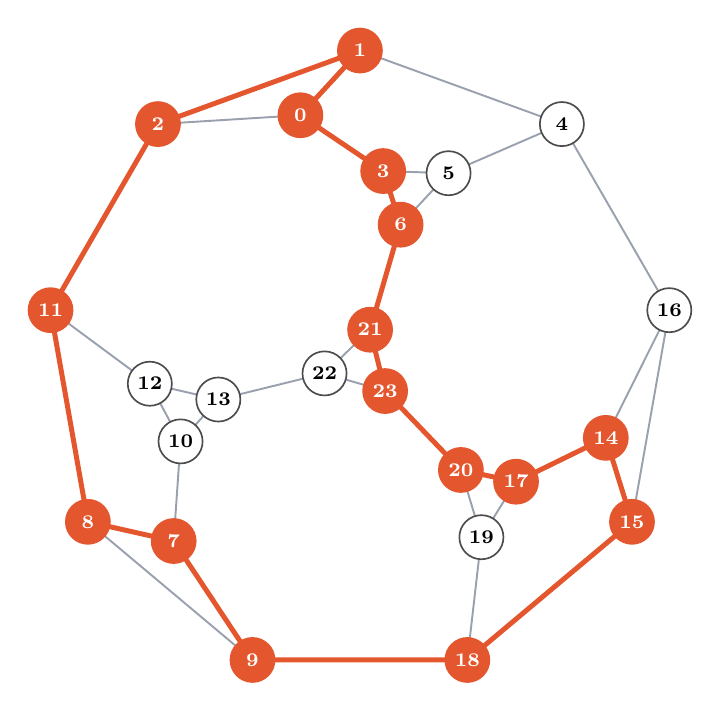
\begin{tikzpicture}[scale=0.95,
    vtx/.style={circle, draw=black!70, fill=white, line width=0.6pt,
                inner sep=0pt, minimum size=5.6mm, font=\scriptsize\bfseries},
    hot/.style={vtx, draw=accent, fill=accent, text=white},
    e/.style={edgegray, line width=0.7pt},
    c/.style={accent, line width=1.8pt, line join=round}]
  % Generated by scripts/draw_markstrom.py layout (Tutte embedding)
\coordinate (v0) at (-0.796,3.335);
\coordinate (v1) at (0.000,4.200);
\coordinate (v2) at (-2.700,3.217);
\coordinate (v3) at (0.311,2.589);
\coordinate (v4) at (2.700,3.217);
\coordinate (v5) at (1.185,2.560);
\coordinate (v6) at (0.544,1.872);
\coordinate (v7) at (-2.490,-2.357);
\coordinate (v8) at (-3.637,-2.100);
\coordinate (v9) at (-1.436,-3.947);
\coordinate (v10) at (-2.398,-1.025);
\coordinate (v11) at (-4.136,0.729);
\coordinate (v12) at (-2.809,-0.254);
\coordinate (v13) at (-1.893,-0.465);
\coordinate (v14) at (3.287,-0.978);
\coordinate (v15) at (3.637,-2.100);
\coordinate (v16) at (4.136,0.729);
\coordinate (v17) at (2.087,-1.564);
\coordinate (v18) at (1.436,-3.947);
\coordinate (v19) at (1.624,-2.306);
\coordinate (v20) at (1.350,-1.407);
\coordinate (v21) at (0.136,0.468);
\coordinate (v22) at (-0.473,-0.116);
\coordinate (v23) at (0.337,-0.352);

  % all edges
  \foreach \u/\v in {0/1,0/2,0/3,1/2,1/4,2/11,3/5,3/6,4/5,4/16,5/6,6/21,
                     7/8,7/9,7/10,8/9,8/11,9/18,10/12,10/13,11/12,12/13,13/22,
                     14/15,14/16,14/17,15/16,15/18,17/19,17/20,18/19,19/20,20/23,
                     21/22,21/23,22/23}
    \draw[e] (v\u) -- (v\v);
  % the 16-cycle
  \draw[c] (v0) -- (v1) -- (v2) -- (v11) -- (v8) -- (v7) -- (v9) -- (v18)
        -- (v15) -- (v14) -- (v17) -- (v20) -- (v23) -- (v21) -- (v6) -- (v3) -- cycle;
  % vertices
  \foreach \v in {0,1,2,3,6,7,8,9,11,14,15,17,18,20,21,23}
    \node[hot] at (v\v) {\v};
  \foreach \v in {4,5,10,12,13,16,19,22}
    \node[vtx] at (v\v) {\v};
\end{tikzpicture}
\caption{The Markstr\"om graph ($n=24$, $m=36$, cubic, planar). The highlighted
vertices and edges form the $16$-cycle from Theorem~\ref{thm:markstrom}.
The three copies of $H_7$ sit at the top, bottom left and bottom right, and
the central triangle $\{21,22,23\}$ connects them.}
\label{fig:markstrom}
\end{figure}

% ===========================================================================
\section{Computational Approach and Python Implementation}\label{sec:code}

\subsection{Overview}

The accompanying program (repository linked on the title page) does three
things:
\begin{enumerate}
  \item builds the Markstr\"om graph and other test graphs from explicit edge
        lists, or reads any graph from a text file;
  \item for each power of two $k\le n$, decides \emph{exactly} whether $G$
        has a $k$-cycle, and if so prints one as a witness;
  \item reports whether the conjecture holds for $G$.
\end{enumerate}

\subsection{The Search Algorithm}

To find a cycle of length $k$, the program runs a depth-limited backtracking
search from every start vertex $s$. It only steps to vertices larger than $s$,
so that each cycle is found from exactly one start, namely its smallest
vertex. It keeps track of the vertices on the \emph{current path} and
un-marks them when it backtracks.

The second point is essential. The original version of this program used a
single ``visited'' set per start vertex. That explores only one DFS tree, so
it misses most cycles. On the Petersen graph, for example, it fails to find
the $8$-cycle, and on $K_4$ it fails to find the $4$-cycle.

\begin{lstlisting}[caption={Exact cycle search (\texttt{src/erdos\_gyarfas/cycles.py}, excerpt).}]
def find_cycle_of_length(graph, k):
    """Return one simple cycle with exactly k vertices, or None."""
    if k < 3 or k > graph.n:
        return None
    adj = [sorted(nbrs) for nbrs in graph.adj]

    for start in range(graph.n):
        if len(adj[start]) < 2:
            continue
        path = [start]
        on_path = [False] * graph.n
        on_path[start] = True
        iters = [iter(adj[start])]      # explicit DFS stack
        while iters:
            advanced = False
            for w in iters[-1]:
                if w < start:
                    continue            # start is the cycle's minimum
                if w == start:
                    if len(path) == k:
                        return list(path)
                    continue
                if on_path[w] or len(path) == k:
                    continue
                path.append(w)          # go deeper
                on_path[w] = True
                iters.append(iter(adj[w]))
                advanced = True
                break
            if not advanced:            # backtrack
                iters.pop()
                on_path[path.pop()] = False
    return None
\end{lstlisting}

\subsection{Sample Output}

Running \texttt{python -m erdos\_gyarfas} produces the following (abridged):

\begin{lstlisting}[language={},numbers=none]
  markstrom
  vertices: 24   edges: 36   min degree: 3
  C4    none
  C8    none
  C16   found   0 -> 1 -> 2 -> 11 -> 8 -> 7 -> 9 -> 18 -> 15 -> 14
                -> 17 -> 20 -> 23 -> 21 -> 6 -> 3 -> 0
  -> conjecture holds for this graph

  petersen
  vertices: 10   edges: 15   min degree: 3
  C4    none
  C8    found   0 -> 1 -> 2 -> 3 -> 4 -> 9 -> 7 -> 5 -> 0
  -> conjecture holds for this graph

  k4
  vertices: 4   edges: 6   min degree: 3
  C4    found   0 -> 1 -> 2 -> 3 -> 0
  -> conjecture holds for this graph

  c7
  vertices: 7   edges: 7   min degree: 2
  C4    none
  -> conjecture does not apply (min degree < 3)
\end{lstlisting}

\subsection{Correctness Checks}

The program comes with an automated test suite. It checks that:
\begin{itemize}
  \item $M$ is cubic, planar, has $24$ vertices and $36$ edges, no $\C4$ or
        $\C8$, and the exact cycle spectrum stated in
        Theorem~\ref{thm:markstrom}, which matches the published
        one~\cite{mathworld};
  \item $K_4$, $K_5$, the Petersen graph, the Heawood graph, the $3$-cube and
        $\C7$ have their known cycle spectra (for instance, the Petersen graph
        has cycles of lengths exactly $5,6,8,9$);
  \item on randomly generated small graphs, the result agrees with a brute
        force check of every vertex subset and every ordering of it.
\end{itemize}
In addition, a separate script re-derives $M$ from the $K_4$/$H_7$ description
alone. It enumerates every gadget matching the description and every way of
wiring it, and finds exactly one cubic planar graph with no $\C4$ and no $\C8$.

\subsection{Complexity}

Deciding whether a graph has a cycle of length exactly $k$ is NP-complete in
general: the case $k=n$ is the Hamiltonian cycle problem. The search above
therefore takes exponential time in the worst case, roughly $O(n\cdot
\Delta^{k-1})$ for maximum degree $\Delta$. For the graphs in this project,
which have at most a few dozen vertices, every query finishes in milliseconds.
Searching for a counterexample at the frontier ($30$ or more vertices, over
all cubic graphs) needs far more sophisticated tools than this program.

% ===========================================================================
\section{Connections to Formal Language Theory}

From the perspective of the LFA course, the conjecture has a natural reading
in terms of languages over a one-letter alphabet.

\begin{itemize}[leftmargin=*]
  \item \textbf{Lengths as unary words.} Identify the number $k$ with the
        word $a^k$. The cycle spectrum of $G$ becomes a language
        $L_G\subseteq a^*$, and the conjecture says that
        $L_G\cap L_2\neq\emptyset$ whenever $\delta(G)\ge3$, where
        \[
          L_2=\{a^{2^k} : k\ge2\}.
        \]
  \item \textbf{$L_2$ is not regular.} Every regular language over a
        one-letter alphabet has an ultimately periodic set of lengths. The gaps
        between consecutive powers of two grow without bound, so $L_2$ is not
        ultimately periodic. Equivalently, the pumping lemma fails: pumping
        $a^{2^k}$ with $2^k\ge p$ by a block of length $1\le j\le p$ gives
        $a^{2^k+j}$, and $2^k<2^k+j<2^{k+1}$. So no finite automaton recognises
        the target set. This is one way to see why arguments that only track a
        bounded amount of information, such as the parity argument of
        Proposition~\ref{prop:even}, cannot settle the conjecture on their own.
  \item \textbf{Graphs as automata.} A graph can be read as a nondeterministic
        automaton over $\{a\}$, with vertices as states and edges as
        transitions. Its closed walks from a vertex $v$ to itself form a
        regular language. Cycles, however, must not repeat vertices, and the
        set of \emph{simple} cycle lengths is not described by the automaton's
        language. This gap between walks and cycles is exactly what makes cycle
        problems hard.
  \item \textbf{Search and the stack.} The search procedure in
        Section~\ref{sec:code} keeps its current path on an explicit stack,
        pushing when it goes deeper and popping when it backtracks, much like a
        pushdown automaton. Unlike a PDA, though, it also needs random access
        to the path to test whether a vertex has already been used.
\end{itemize}

% ===========================================================================
\section{Conclusion}

The Erd\H{o}s--Gy\'arf\'as Conjecture is easy to state yet sits at the
frontier of graph theory. In this paper we:
\begin{enumerate}
  \item placed the conjecture in its historical context;
  \item developed the necessary background, and proved that minimum degree $3$
        forces an even cycle, though not a cycle of any particular length;
  \item summarised the known partial results, including the planar cubic case
        and the large-minimum-degree theorem of Liu and Montgomery;
  \item gave an explicit construction of the Markstr\"om graph, drew it, and
        verified its key properties;
  \item presented and tested an exact search program for power-of-two cycles;
  \item related the problem to unary languages and the non-regularity of
        $\{a^{2^k}\}$.
\end{enumerate}
The case of small minimum degree, and of cubic graphs in particular, remains
wide open. Its resolution will likely need new structural ideas, or a
computer-assisted search far larger than any carried out so far.

% ===========================================================================
\begin{thebibliography}{99}

\bibitem{bondy-simonovits}
J.~A. Bondy and M.~Simonovits.
\newblock Cycles of even length in graphs.
\newblock \emph{Journal of Combinatorial Theory, Series B}, 16(2):97--105, 1974.

\bibitem{dirac}
G.~A. Dirac.
\newblock Some theorems on abstract graphs.
\newblock \emph{Proceedings of the London Mathematical Society}, s3-2(1):69--81,
  1952.

\bibitem{erdos1997}
P.~Erd\H{o}s.
\newblock Some old and new problems in various branches of combinatorics.
\newblock \emph{Discrete Mathematics}, 165--166:227--231, 1997.
\newblock \doi{10.1016/S0012-365X(96)00173-2}.

\bibitem{erdosproblems}
T.~F. Bloom.
\newblock Erd\H{o}s Problem \#64.
\newblock \url{https://www.erdosproblems.com/64}, accessed October 2026.

\bibitem{heckman-krakovski}
C.~C. Heckman and R.~Krakovski.
\newblock Erd\H{o}s--Gy\'arf\'as conjecture for cubic planar graphs.
\newblock \emph{Electronic Journal of Combinatorics}, 20(2):\#P7, 2013.
\newblock \doi{10.37236/3252}.

\bibitem{liu-montgomery}
H.~Liu and R.~Montgomery.
\newblock A solution to Erd\H{o}s and Hajnal's odd cycle problem.
\newblock \emph{Journal of the American Mathematical Society}, 2023.
\newblock \doi{10.1090/jams/1018}.

\bibitem{markstrom}
K.~Markstr\"om.
\newblock Extremal graphs for some problems on cycles in graphs.
\newblock \emph{Congressus Numerantium}, 171:179--192, 2004.

\bibitem{three-graphs}
G.~Exoo.
\newblock Three graphs and the Erd\H{o}s--Gy\'arf\'as conjecture.
\newblock arXiv:1403.5636.

\bibitem{tutte}
W.~T. Tutte.
\newblock How to draw a graph.
\newblock \emph{Proceedings of the London Mathematical Society}, s3-13:743--767,
  1963.

\bibitem{mathworld}
E.~W. Weisstein.
\newblock Markstr\"om graph.
\newblock \emph{MathWorld}, \url{https://mathworld.wolfram.com/MarkstroemGraph.html}.

\end{thebibliography}

\end{document}
